%
% File emnlp2018.tex
%
%% Based on the style files for EMNLP 2018, which were
%% Based on the style files for ACL 2018, which were
%% Based on the style files for ACL-2015, with some improvements
%%  taken from the NAACL-2016 style
%% Based on the style files for ACL-2014, which were, in turn,
%% based on ACL-2013, ACL-2012, ACL-2011, ACL-2010, ACL-IJCNLP-2009,
%% EACL-2009, IJCNLP-2008...
%% Based on the style files for EACL 2006 by
%% e.agirre@ehu.es or Sergi.Balari@uab.es
%% and that of ACL 08 by Joakim Nivre and Noah Smith

\documentclass[11pt,a4paper]{article}
\usepackage[hyperref]{emnlp2018}
\usepackage{times}
\usepackage{latexsym}
\usepackage{url}
\usepackage{mathptmx} 
\usepackage{amsmath}


\aclfinalcopy % Uncomment this line for the final submission

%\def\aclpaperid{***} %  Enter the acl Paper ID here

%\setlength\titlebox{5cm}
% You can expand the titlebox if you need extra space
% to show all the authors. Please do not make the titlebox
% smaller than 5cm (the original size); we will check this
% in the camera-ready version and ask you to change it back.

\usepackage{graphicx}
\graphicspath{{figures/}{pictures/}{figs/}{./}} % where to search for the images
\usepackage{xcolor}  % Coloured text etc.
\usepackage{listings}
%\usepackage{authblk}

\definecolor{codegreen}{rgb}{0,0.6,0}
\definecolor{codegray}{rgb}{0.5,0.5,0.5}
\definecolor{codepurple}{rgb}{0.58,0,0.82}
\definecolor{backcolour}{rgb}{0.95,0.95,0.92}
\lstdefinestyle{mystyle}{
    %backgroundcolor=\color{backcolour},   
    commentstyle=\color{codegreen},
    keywordstyle=\color{magenta},
    numberstyle=\tiny\color{codegray},
    stringstyle=\color{codepurple},
    basicstyle=\scriptsize\ttfamily\bfseries,
    %basicstyle=\footnotesize\ttfamily,
    breakatwhitespace=false,         
    %breaklines=true,                 
    captionpos=b,                    
    keepspaces=true,                 
    %numbers=left,                    
    %numbersep=1pt,                  
    showspaces=false,                
    showstringspaces=false,
    showtabs=false,                  
    tabsize=1
}

\lstset{style=mystyle}

\newcommand\BibTeX{B{\sc ib}\TeX}
\newcommand\confname{EMNLP 2018}

\title{Visual Interrogation of Attention-Based Models: \\ Applications in Language Inference and Machine Comprehension}

\author{Shusen Liu$^{1}$, Tao Li$^{2}$,  Zhimin Li$^{3}$,  Vivek Srikumar$^{2}$, Valerio Pascucci$^{3}$, Peer-Timo Bremer$^{1}$ \\
 % {\tt liu42@llnl.gov} \\\And
  Lawrence Livermore National Laboratory$^{1}$\\
  School of Computing, University of Utah$^{2}$\\  
  SCI Institute, University of Utah$^{3}$\\
   % {\tt {tao.li, zhimin.li, vivek, pacucci}@utah.edu}
} 

%\date{}
\begin{document}
\maketitle

%\vspace{-4mm}

\begin{abstract}
Neural networks models have gained unprecedented popularity in natural language processing due to their state-of-the-art performance and the flexible end-to-end training scheme. Despite their advantages, the lack of interpretability hinders the deployment and refinement of the model.
%These models often relying on the attention mechanism, which not only helps improve predicting performance but also provide interpretable representations for users to peak into the opaque models that are usually considered as black boxes.
%
In this work, we present a flexible visualization library for creating customized visual analytic environments, in which the user can investigate and interrogate the relationship among the input, the model internals (i.e., attention), and the output predictions that in turn shed light on the model decision making processing.
 
\end{abstract}


Outline
\begin{itemize}
    \item the important of LSTM/RNN
    \item the criptic natural of the hidden state, where a single state represents the whole sequence
    \item the need to understand how does the model remember and forget? especially in analysis long sequence in the real world scenarios
    \item Understand how the gate affect the prediction
\end{itemize}

Many recent advances of neural language processing is driven by the continoues evolving and improving of the recurrent neural networks. These model processes information in a sequenctial fashion, which can easily handle the flexible and variable length


The, recently several visualization work has focused on visualizing the recurrent neural network such as the long-short term memory (LSTM) network

\section{Related Works}


Visualizing and understanding neural models in nlp
Understanding Neural Networks through Representation Erasure
Interactive Visualization and Manipulation of Attention-based Neural Machine Translation
End-to-End Non-Factoid Question Answering with an Interactive Visualization of Neural Attention Weights

%\subseciton{other}
DeepLife: an Entity-aware Search, Analytics and Exploration Platform for Health and Life Sciences
Visualizing and Curating Knowledge Graphs over Time and Space
GoWvis: a Web Application for Graph-of-Words-based Text Visualization and summarization
new/s/leak - Information Extraction and Visualization for an Investigative Data Journalists
Multi-modal Visualization and Search for Text and Prosody Annotations
Visual Error Analysis for Entity Linking
JoBimViz: A Web-based Visualization for Graph-based Distributional Semantic Models
WA-Continuum: Visualising Word Alignments across Multiple Parallel Sentences Simultaneously
Scattertext: a Browser-Based Tool for Visualizing how Corpora Differ
Interactive Visual Analysis of Transcribed Multi-Party Discourse
Visualization, Search, and Error Analysis for Coreference Annotations


\begin{figure}[htbp]
\centering
\vspace{-2mm}
 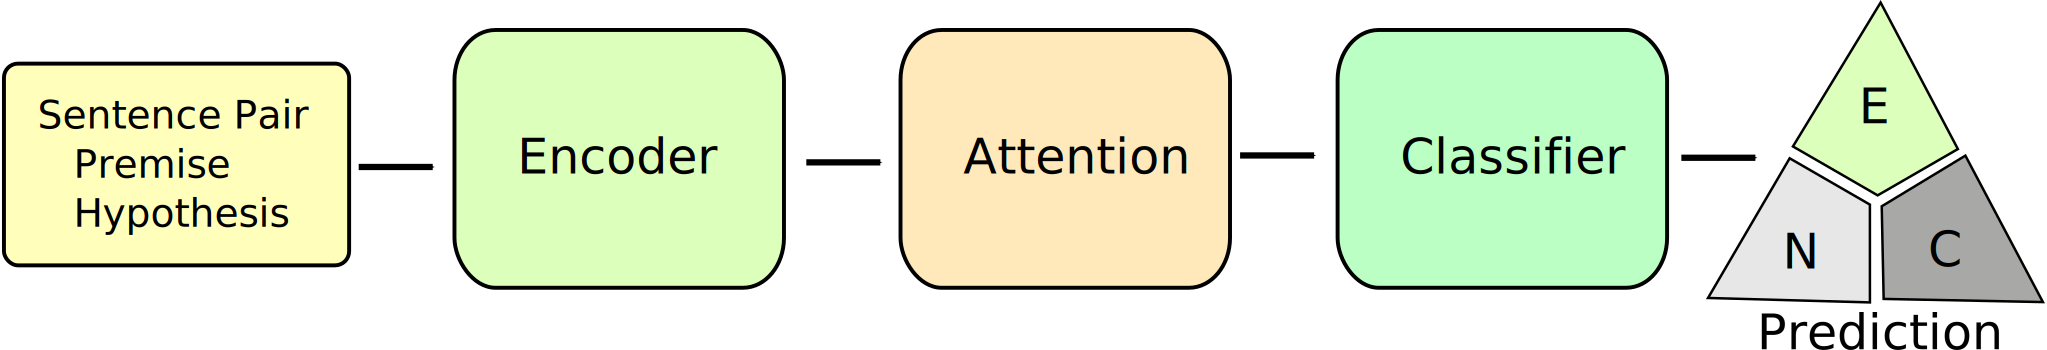
\includegraphics[width=1.0\linewidth]{pipeline}
 \caption{
 Perturbation-driven exploration of the end-to-end models that follows the encoder, attention, and classifier structure. The user can generate small perturbation of the input (i.e., replacing synonyms, paraphrasing)
 }
\label{fig:modelPipeline}
\end{figure}

\section{Visualization System}
As illustrated in Figure~\ref{fig:modelPipeline}, many recent end-to-end NLP model follows a similar encode, attent, and classify structure, in which the attention stage provide a window for peeking into the model decision making process. However, the static attention alone likely does not tell the whole story, instead we can learn more about the model by examining the dynamic between the input, the attention, and the output. To explore the relationship between different components of the pipeline, the proposed system utilizes a perturbation-driven exploration strategy, where the  user can manually or automatically generate small changes in the input sentence and then view the aggregated prediction information. Beside the perturbation of the input, the system also allows interactive modification of the attention values, where the prediction will instantaneously updated to reflect the changes. 
%

\subsection{Input Sentences Perturbation}
\label{sec:perturb}
Due to the discrete nature of the natural language, applying perturbation to sentence for sensitivity analysis can be particularly challenging compared to other problem domain, as small changes in words can leading to drastic different in the semantics of the sentences.
To reduce the potential semantic deviation, we first devise a simple perturbation method by replacing \emph{nouns} and \emph{verbs} by their synonyms in the wordNet~\cite{Miller1995}. However, the limitation is apparent, as synonyms replacement does not guarantee the meaning of the sentence remain the same. And the wordNet also has a rather inclusive definition for synonyms, where many infrequent/obscure usages exists, which leads to less meaningful perturbed sentence. However, this method requires minimal computation and easy to code and understand. 

\begin{figure}[htbp]
\centering
\vspace{-2mm}
 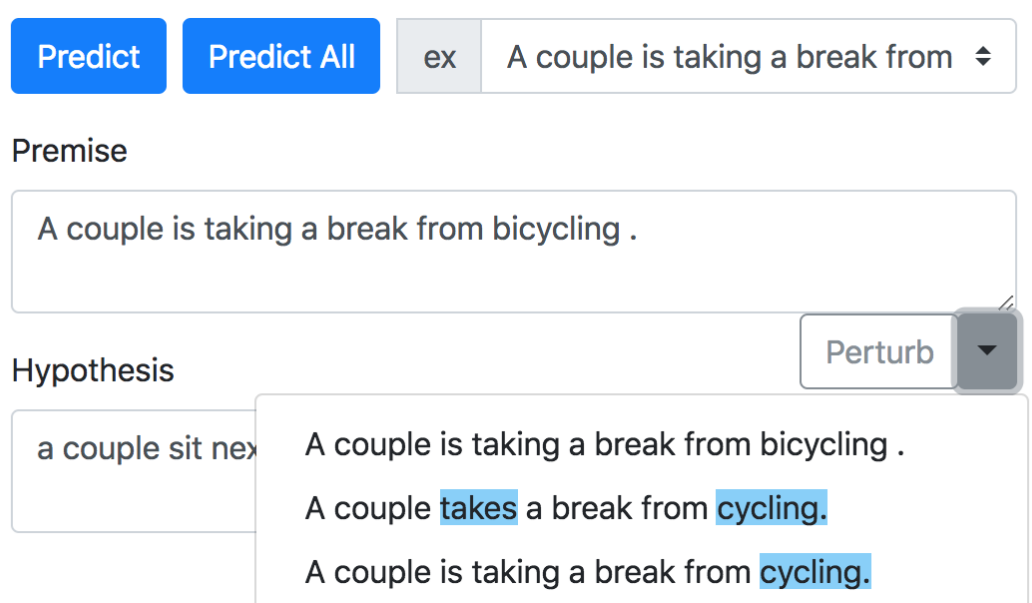
\includegraphics[width=0.9\linewidth]{sentence}
 \caption{
The interface for showing input sentences. The user can manually alter the words or apply automatic perturbation/paraphrasing of the inputs. In the \emph{perturbed} dropdown menu, the blue words are the only not exist in the original sentence.
 }
\label{fig:sentence}
\end{figure}

To improve the perturbation quality, we also adopted a translation based paraphrasing technique that is similar to the method discussed in \cite{mallinson2017paraphrasing}. Here, we translate the original English sentence into several other languages are then translate back into the English. Provided the translation produce correct result, we essential obtain paraphrasing of the original sentences (see Figure~\ref{fig:sentence}, where the drop-down menu shows the paraphrased/perturbed sentence).

\begin{figure}[htbp]
\centering
\vspace{-2mm}
 \includegraphics[width=0.8\linewidth]{prediction}
 \caption{
Summarize the prediction results of the perturbed input for the natural language inference model.
the prediction is encoded as a point in the barycentric coordinate system of the triangle, in which each vertex corresponds to one prediction label, namely, \emph{entail}, \emph{contradict}, and \emph{neutral}.
 %
 }
\label{fig:prediction}
\end{figure}


\subsection{Prediction Visualization}

The prediction result for the original sentence pair is represented by a larger yellow circle and the prediction of perturbed pairs are illustrated by smaller grey circles.

A density contour of the prediction is computed to emphasize the highly cluttered areas and distinguish the outliers.

\begin{figure*}[t]
\centering
\vspace{-2mm}
 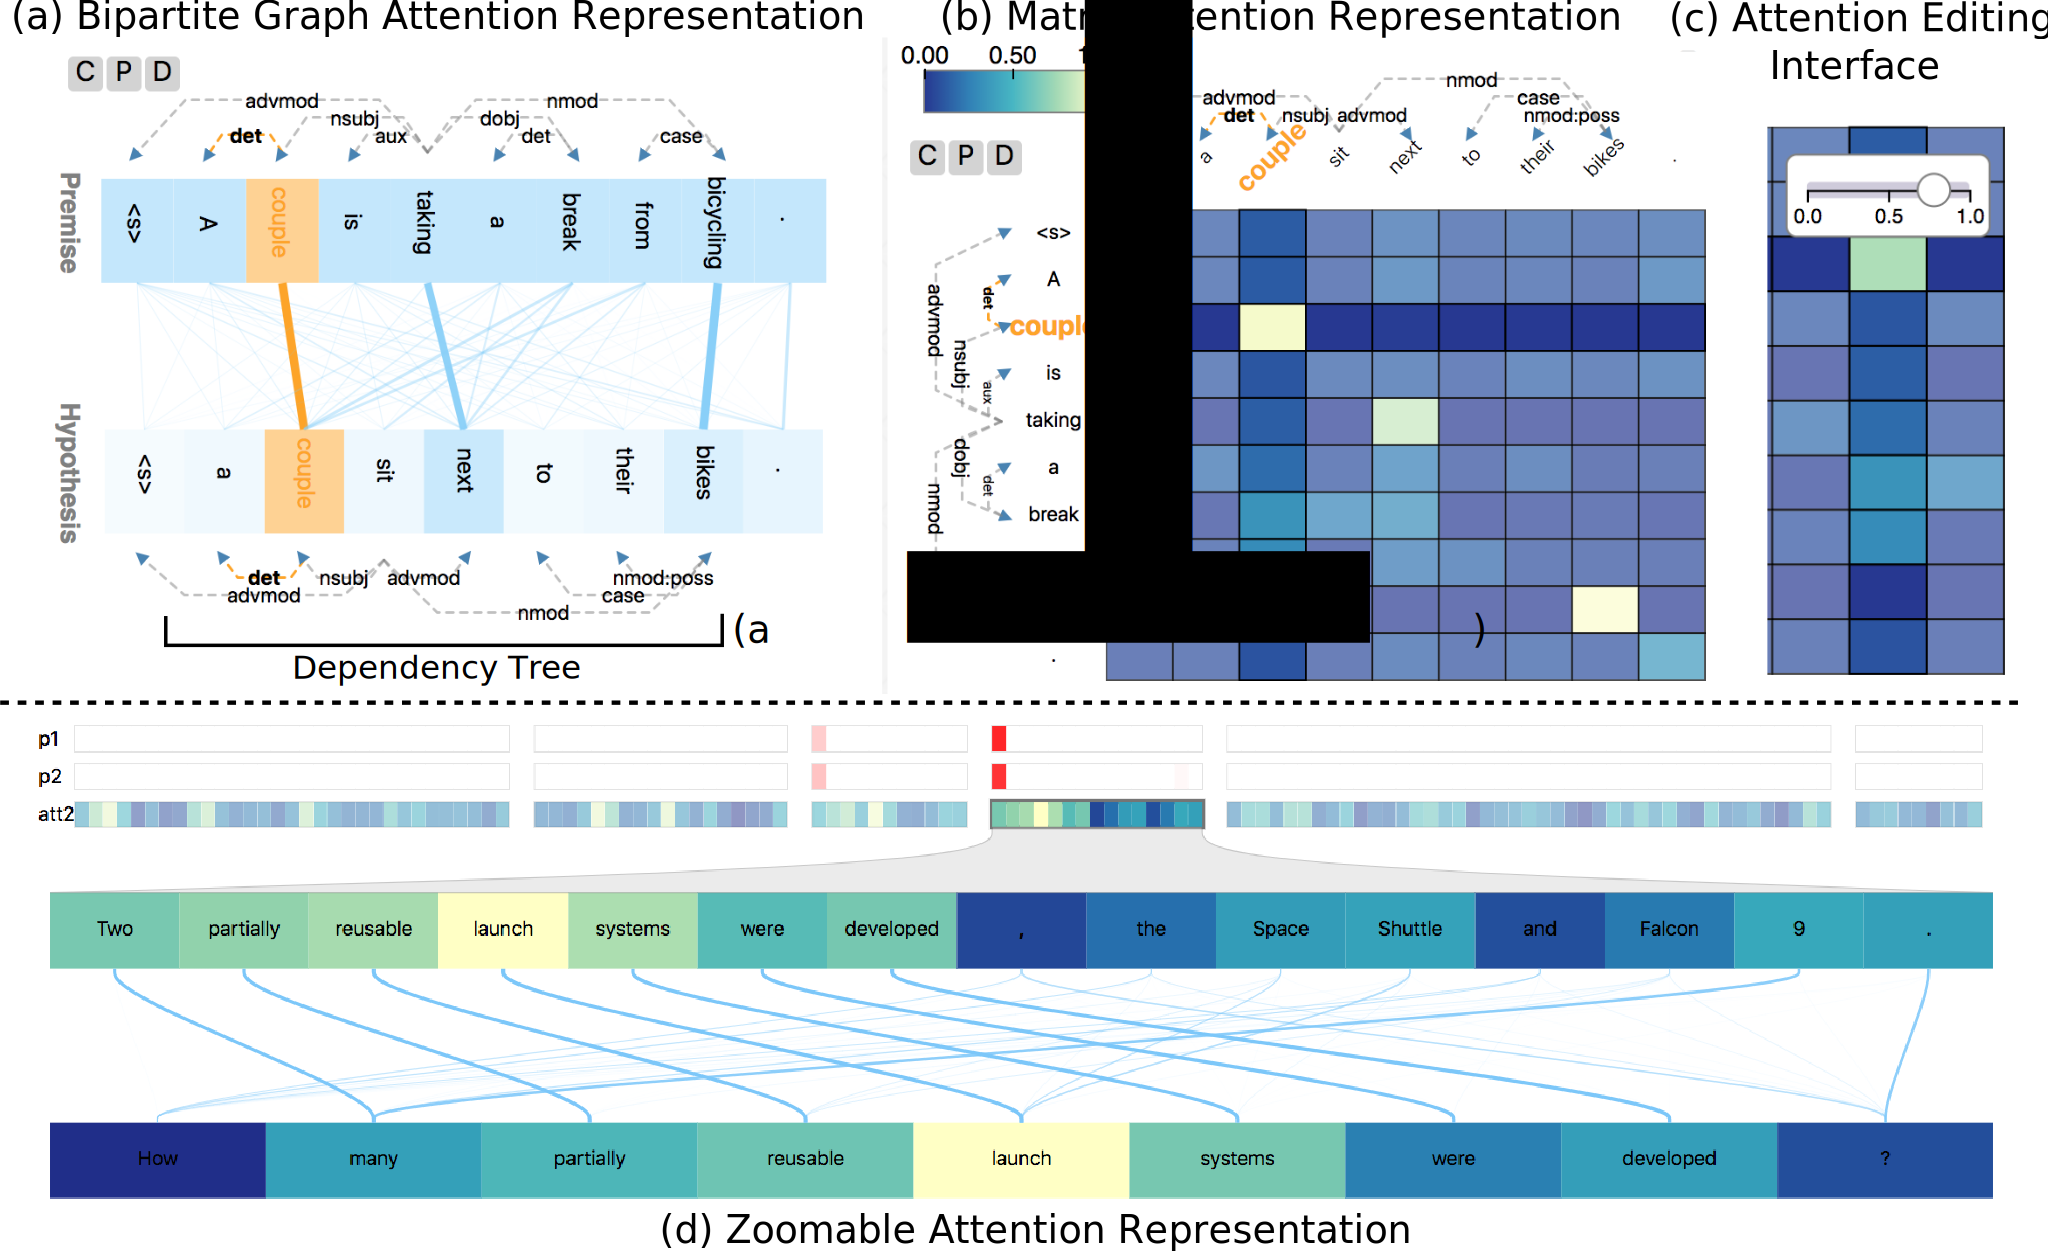
\includegraphics[width=0.9\linewidth]{attentionPanels}
  \vspace{-3mm}
 \caption{
Attention visualization. In the graph attention view (a), a bipartite graph encoding is adopted, in which the edge thickness corresponds to the attention value. In the matrix attention view (b), the entries of $i^{th}$ row represent the probabilities of words in hypotheses align to the $i^{th}$ word in the premise.
The user can alter the attention values via the pop-up interface illustrated in (c).
We overlay the dependency tree ($a_1$) grammar structure to highlight important words and allow simplification of complex sentence based on the dependency tree.
%
For highly asymmetric attention relationship, we utilized a zoomable hierarchical visual representation (d).
}
\label{fig:attentionVis}
\end{figure*}

\subsection{Attention Visualization}
The system consistence several visualization components that can be combine to generate an functional interactive system. Here we will focus on the attention visualization components. 
As illustrated in Figure~\ref{fig:attentionVis}(a)(b), the most widely adopted technique to bipartie graph (a), as well as the heatmap attention matrix representation (b). 
%
In the graph attention view (Fig.~\ref{fig:attentionVis}(a)), a bipartite graph encoding is adopted, in which the edge thickness corresponds to the attention value. The color of the rectangle text block encodes the sum of all edge values connected to it (darker shade of blues correspond to higher values).
%%%%%%%%
The graph view is suitable for highlighting the most dominant alignments. However, the edges may become cluttered if multiple attention values are high. The matrix attention view (Fig.~\ref{fig:attentionVis}(b)) resolve these issues, despite being more verbose and less efficient in highlighting the dominant alignments. 
%Together, the graph and matrix views complement each other and provide the same information from different perspectives. As illustrated by the pink arrowed lines, we can see how the same attention value is visualized in both the graph and the matrix view.
To help the user recognize the correspondence during the exploration, we enable the linkage between highlighted actions in both views (see Fig.~\ref{fig:attentionVis}(a)(b), the attention of the two ``couple'' is highlighted).
%
To address the challenge of visualizing long sentence, we incorporated the grammar structure.
One augmentation 

However, when the one of the text sequence become signification 

\subsection{Implementation}
The initial setup cost and learning curve of the tool are often the barriers for user adaptation. To address these challenge, we design the visualization system as a Python library with modularity and easy accessibility in mind.
Instead of using the visualization system as a monolithic standalone application, just like a plotting library (i.e., matplotlib), the different pieces of the visualization (i.e., matrix based attention encoding) can be accessed individually.
% 
Yet, the components can also be combined in any configuration desired by users via a simple API to better fit into one's workflow.
More importantly, the library-based design allows easy integration with the existing model implemented in Python.
%
To create a visualization, users only need to import the library, create an instance of the visualization object, and specify a set of callback functions, such as generating a prediction, accessing attention, to link the visualization to their NLP models. The the code required to create an interactive exploration environment for machine comprehension model is illustrated bellow.

\begin{lstlisting}[language=Python, caption=Code for setting up the visualization system shown in the paper.]
from visPackage import MCModule
from bidaf_src import bidafModelInterface
from NLPutility import translationPerturbation

#initialize machine comprehension model
model = bidafModelInterface(
    wordDict="data/bidaf/squad.word.dict",
    wordVec="data/bidaf/glove.hdf5",
    model="data/bidaf/bidaf.ema")
gen = translationPerturbation()
#visualization components
visLayout = {
  "column":[{"row": ["Paragraph", 
                     "AttentionSubMatrix"]},
            {"row": ["AttentionAsymmetric"]}]
  }
#setup interface
modelVis = MCModule(visLayout)
modelVis.setPredictionHook(model.predict)
modelVis.setAttentionHook(model.attention)
modelVis.setSentenceHook(gen.perturbSentence)
#open browser for the web-based visualization
modelVis.show()
\end{lstlisting}





\begin{figure*}[t]
\centering
\vspace{-2mm}
 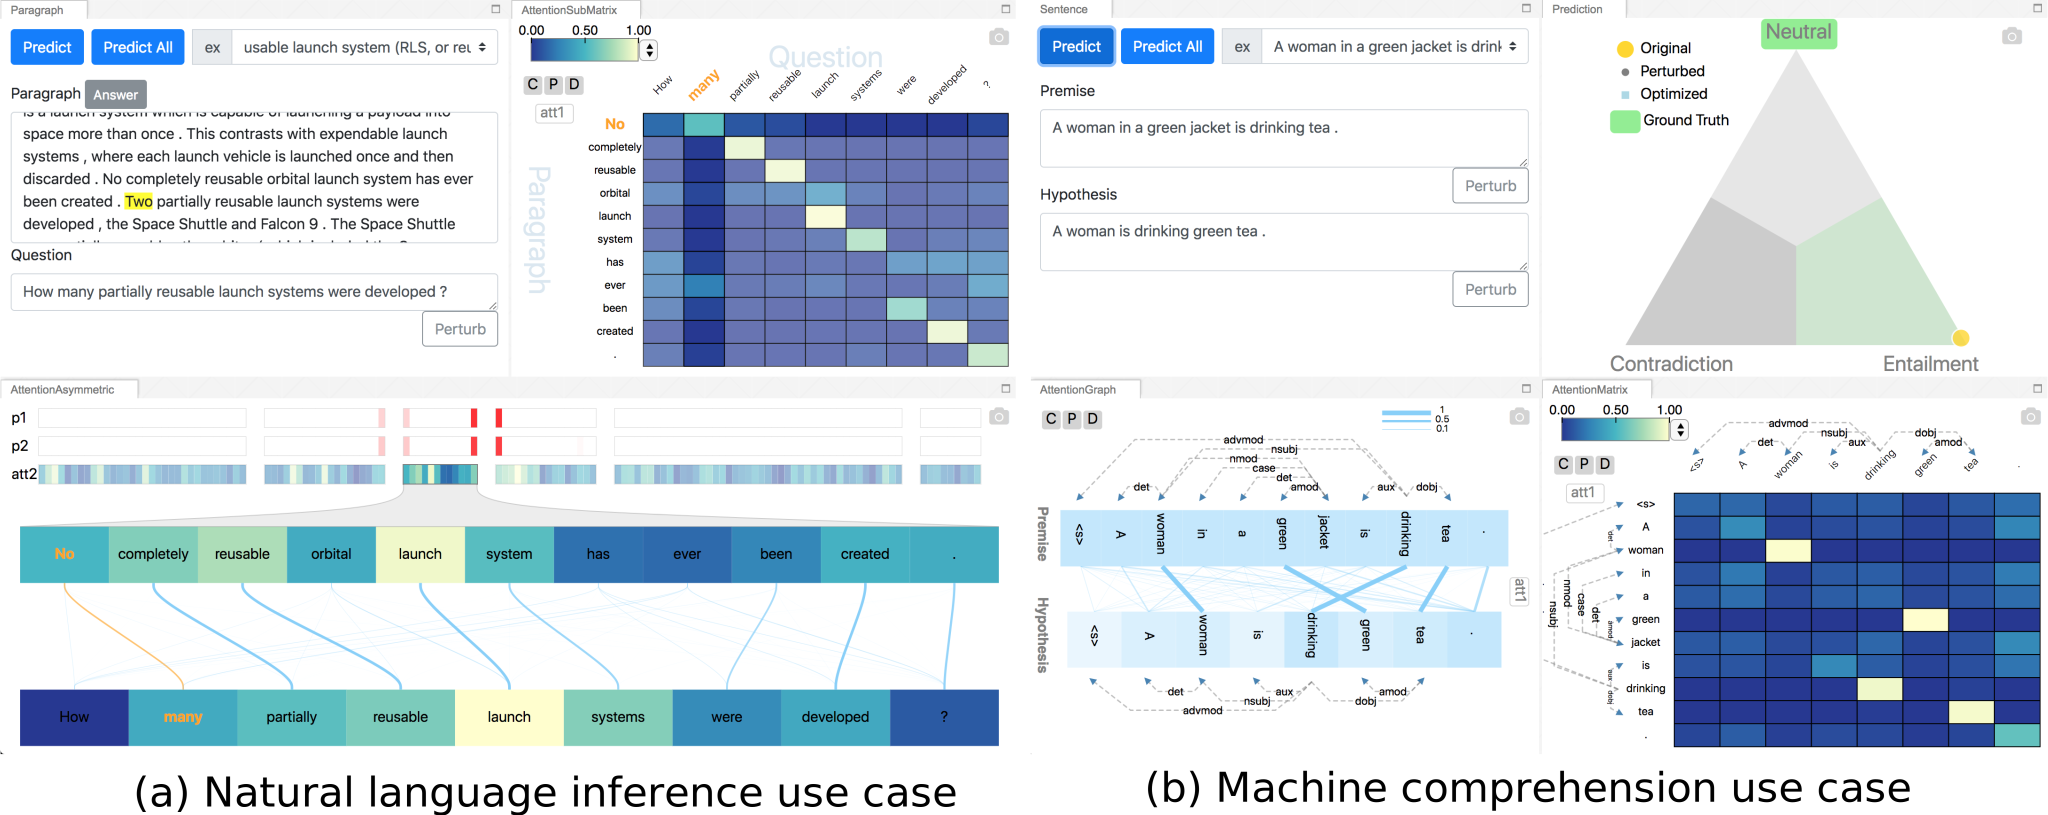
\includegraphics[width=1.0\linewidth]{NLI_MC_interface}
  \vspace{-6mm}
 \caption{
Illustration of different configurations for the natural language inference and machine comprehension tasks.
}
\label{fig:pipelineUpdate}
\end{figure*}

\section{Application Results}


\subsection{Natural Language Inference}
We demonstrate our visualization system on the decomposable attention networks
for NLI task. The goal is that, given a premise sentence and a hypothesis sentence,
predict their relation as one of \emph{Entailment, Contradiction, Neutral}.
The model can be formalized as the following:
\begin{align}
	P^\prime, H^\prime &= f(P), f(H)\\
	\overleftarrow{A} &= P^\prime \cdot H^\prime\\
	\overrightarrow{A} &= H^\prime \cdot P^\prime\\
	y &= g(P, H, P^\prime, H^\prime, \overleftarrow{A}, \overrightarrow{A})
\end{align}
where $P$ and $H$ are input embedding matrices for the premise and the hypothesis, $\overleftarrow{A}$
and $\overrightarrow{A}$ are attentions, and $y$ is the predicted probabilities for candidate classes.
Our system visualized the bidirectional attentions and their interaction with output distribution over labels.


\subsection{Machine Comprehension}
In machine comprehension task, two sequences of texts are given: context and question.
The target is to select a span of text from the context that answers the question. We provide a simple model
formulation and refer the reader to the paper for details.
\begin{align}
	C^\prime, Q^\prime &= BiLSTM(C), BiLSTM(Q)\\
	\overleftarrow{A} &= u(C^\prime, Q^\prime)\\
	\overrightarrow{A} &= v(C^\prime, Q^\prime)\\
	s &= m(C^\prime, Q^\prime, \overleftarrow{A}, \overrightarrow{A})\\
	e &= n(s, C^\prime, Q^\prime, \overleftarrow{A}, \overrightarrow{A})
\end{align}
where $C$ and $Q$ are embedding matrices for the context and the question,
$\overleftarrow{A}$ and $\overrightarrow{A}$ are bidirectional attention flows,
$s$ and $e$ are probabilities for starting and ending indices of the answer span.
Our system reveals the internal states of $\overleftarrow{A}$, $\overrightarrow{A}$,
$s$ and $e$.

\section{Discussion}
In this work, we introduce a visualization library for creating customized environments that allow the user to interrogate the relationship between different parts of the model pipeline via interactive queries.
%
We demonstrate the usability and flexibility of the tool by configuring the visual components to investigate models for different NLP tasks (e.g., NLI, MC).
%
We also conducted a small-scale user evaluation, in which five Ph.D. level students with NLP background spent 30 minutes with the tool and then provided feedback. Most suggested the environment allowed them to refine queries iteratively and identify potential issues with the model, but some also mentioned the tool might not provide enough guidance for users who do not have an in-depth understanding of the model at hand.

Even though we designed the individual components with versatility in mind, due to a large number of variants of attention networks, it is hard to ensure compatibility with all the available configurations.
%
In the future, we plan to improve upon the current attention interface, release the library as an open-source package, and expand the visualization components to handle tasks such as neural machine translation and more.


\bibliographystyle{acl_natbib_nourl}
\bibliography{NLPvis.bib}

\end{document}
